
\title{Recap Computer System Security (02KRQOV)}
\author{Jacopo Nasi\\
        Computer Engineer\\
        Politecnico di Torino}
\date{I Period - 2018/2019\\\bigskip\bigskip\today}

\documentclass[12pt]{article}
\usepackage[utf8]{inputenc}
\usepackage[english]{babel}
\usepackage{geometry}
\usepackage{indentfirst} % First line indent
\usepackage{mathtools}
\usepackage{wrapfig}
\usepackage[usenames, dvipsnames]{color}
\usepackage{float}
\usepackage{amssymb}
\usepackage{ifsym}
\usepackage{listings}
\usepackage{multicol}

% Misure Documento
\geometry{ a4paper, total={170mm,257mm},left=35mm, right=35mm, top=35mm, bottom=35mm }

\begin{document}

\begin{figure}
  \centering
  
\includegraphics[width=10cm]{images/polito.pdf}
\end{figure}

\maketitle


\newpage
\tableofcontents

\newpage
{\noindent \Large \textbf{License}\bigskip}

This work is licensed under a Creative Commons Attribution-NonCommercial-ShareAlike 3.0 Unported License.\\
You are free:
\begin{itemize}
  \item \textbf{to Share}: to copy, distribute and transmit the work
  \item \textbf{to Remix}: to adapt the work
\end{itemize}
Under the following conditions:
\begin{itemize}
  \item \textbf{Attribution}: you must attribute the work in the manner specified by the author or licensor (but not in any way that suggests that they endorse you or your use of the work)
  \item \textbf{Noncommercial}: you may not use this work for commercial purposes.
  \item \textbf{Share Alike}: if you alter, transform, or build upon this work, you may distribute the resulting work only under the same or similar license to this one.
\end{itemize}

\noindent More information on the Creative Commons website (http://creativecommons.org).

\begin{figure}[h!]
  \centering
  
\includegraphics[width=3cm]{images/license.png}
\end{figure}

{\noindent \Large \textbf{Acknowledgments}\bigskip}

Questo breve riepilogo non ha alcuno scopo se non quello di agevolare lo studio di me stesso, se vi fosse di aiuto siete liberi di usarlo.\\
Le fonti su cui mi sono basato sono quelle relative al corso offerto (\textbf{Computer System Security (02KRQOV)}) dal Politecnico di Torino durante l'anno accademico 2018/2019.\\
Non mi assumo nessuna responsabilità in merito ad errori o qualsiasi altra cosa. Fatene buon uso!
\newpage

\section{Introduction Security ICT System}
\textbf{Why is securoty an important issue?} Nowadays that everything is online and connected to a world wild network, the security over the ICT system has become fundamental. A lack of the secutiry could generate lose for milions of money. Also data breach become a problem.\\
Everydays technology improve and drive innovation but security must be improved together with the innovations.\\
With the increase of the number of connected devices, the IoT (Internet of Things), security start to facing a lot of more problem, the complexity of the scenario has become really really big. From personal devices, like desktop, laptop, fridge or car, by communications networks, and to distributed services, everything must be secured!\\
\paragraph{Complexity enemy of security} based on one of the first axiom of engineering: \textit{"The more complex a syste, is, the more difficult its correctness verification will be."}. Keep a system as simple as possible is always a good idea. The KISS rules (\textbf{\textit{Keep It Simple, Stupid}}) is one of the most important rule over the system security.
\paragraph{Definition of ICT Security}

\bigskip
``It is the set of products, services, organization rules and individual behaviours that protect the ICT system of a company.\\

It has the duty to protect the resources from undesired access, guarantee the privacy of information, ensure the service operation and availability in case of unpredictable events (C.I.A. = Confidentiality, Integrity, Availability).\\

The objective is to guard the information with the same professionalism and attention as for the jewels and deposit certificates stored in a bank caveau.\\

The ICT system is the safe of our most valuable information; ICT security is the equivalent of the locks, combinations and keys required to protect it.''\\
\rightline{{\rm --- \textbf{Italian Bank}}}
\bigskip

An important part of the security study is the Risk Estimation, is a fundamental step that take in account all the assets and events to evaluate the risk of something. The flow is showed in figure \ref{fig:risk_est}:

\begin{figure}[h!]
  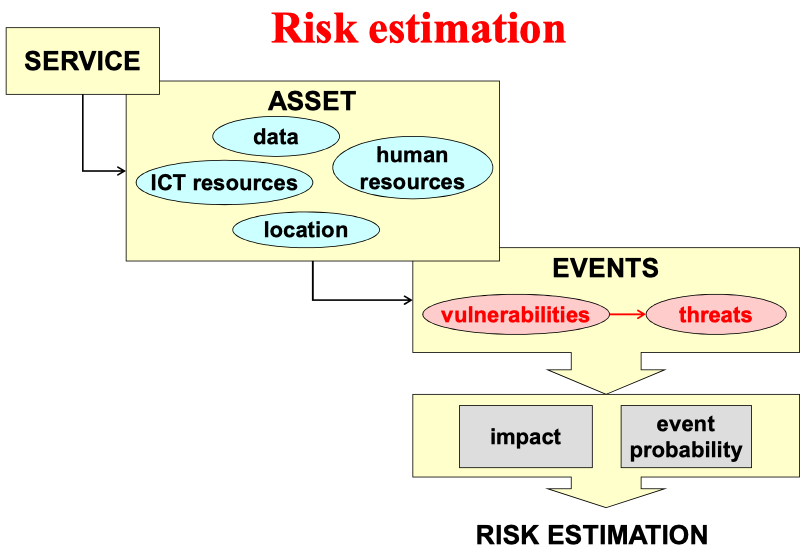
\includegraphics[width=\linewidth]{images/risk_est.png}
  \caption{Risk Estimation}
  \label{fig:risk_est}
\end{figure}

Where the assets is composed by everythings needed by a service to work, both soft and hard part, also human resources. The vulnerabilities, intrinsic of an asset, represent the weakness of it. The threats is a deliberate action, or an accidental event, that can produce the loss of a security properties exploting a vulnerability. The event is also characterized by an impact and a probability that could be high, low or other middle values.\\
Direct following of the risk estimation is the Analysis and management of security. After the evaluation of risks, is necessary to:
\begin{enumerate}
  \item Select Countermeasures
  \item Implement Countermeasures
  \item Audit (check if works)
\end{enumerate}

The security implement is not a phase of the developmente process, is part of each sigle part of it. Security can't be compute at the end of the development, it must be implement from the beginning of the process. \textbf{Security is a process, not a product!} The following figure \ref{fig:dev} show the parallel line followed by the security development.

\begin{figure}[h!]
  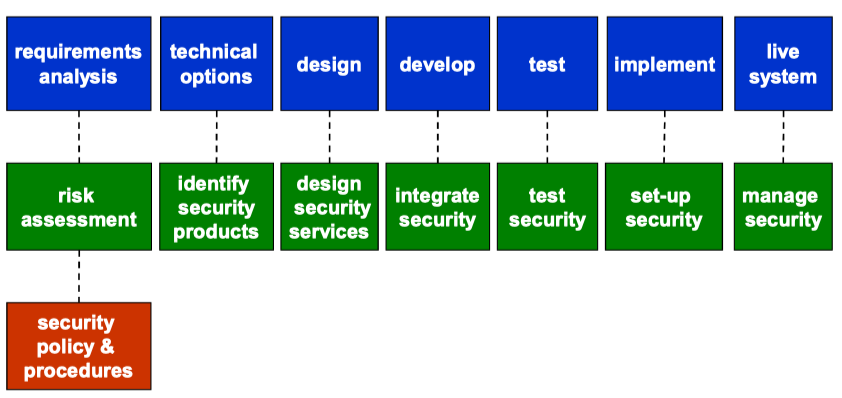
\includegraphics[width=\linewidth]{images/dev.png}
  \caption{Security Life Cycle}
  \label{fig:dev}
\end{figure}

An important definition, before speaking about security itself, is the \textbf{Window of Exposure} the represent the time when an attack could be perfomed and there are no countermeasures to avoid it. This window could potentially be infinite and this is the real problem.
The figure \ref{fig:window} show how this windows id divided in different part:

\begin{figure}[h!]
  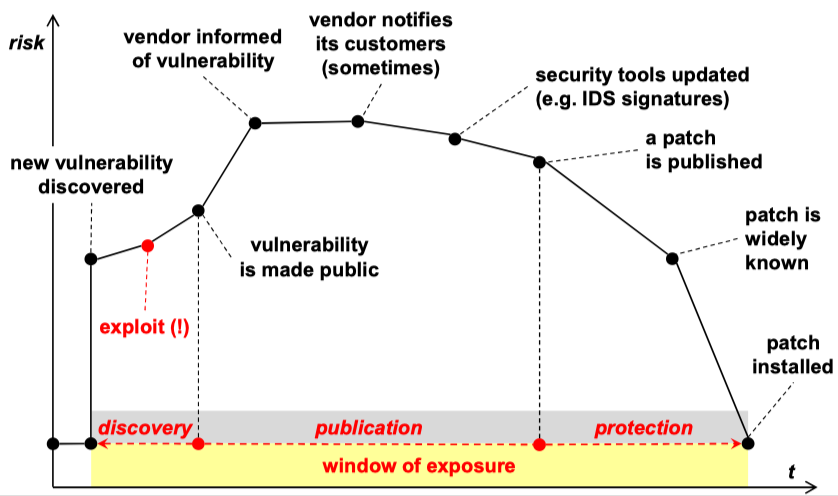
\includegraphics[width=\linewidth]{images/window.png}
  \caption{Window of Exposure}
  \label{fig:window}
\end{figure}

As already says, security is not a product but is a proccess. Computer flaws are inevitable and this is way we can't use devote our security to only secured products. The only way to effectively do business is an insecure world is to put processes in place that recognize the inheritent insecurity in the products. \textbf{The trick is to reduce your risk of exposure regardless of the products or patches}.

\paragraph{Security Principles} Here some of the most important security principles:
\begin{itemize}
  \item Security by Design
  \item Least Privilege: Only correct rights and the only few needed
  \item Need-to-know: Access to the only piece of stuff that are needed
  \item Security by Default
  \item Security in Depth: More the importance of the system, more the obstacles
\end{itemize}

\paragraph{Security Properties} The following list show the most importante properties of the security world:
\begin{itemize}
  \item Authentication (Simple/Mutual): Source (or both) must prove themself
  \item Data Origin/Authentication
  \item Authorization and Access Control
  \item Confidentiality/Privacy/Secrecy
  \item Non Repudiation: Formal proof, acceptable by a court of justice, that gives undeniable evidence of the data creator
  \item Availability
  \item Accountability
  \item Integrity: Modification, Filtering
\end{itemize}

\paragraph{Where is the enemy?} The enemy normally is supposed to be outside of our system but is not simple as it seems. The possible locations are:
\begin{itemize}
  \item Outside our organization (Firewall)
  \item Outside our organization, with exceptionn of our parters (VPN)
  \item Inside our organitazion
  \item Everywhere!
\end{itemize}
The last item is probably the more true. The distinction between internal/external and good/bad guys is no more sufficent. From the \textit{Verizon Data Breach Invetigation Report} the percentage of source of attacks is: 20\% Internal and 80\% External, probably the internal percentage is a little bit higher due to the fact that Verizon is a provider and can't show the internal side so much.

\paragraph{Basic Problems} There are some basic problem for security:
\begin{itemize}
  \item Networks are insecure:
  \begin{itemize}
    \item Clear communications
    \item LAN use broadcast
    \item Not E2E geographical connections
  \end{itemize}
  \item Weak user Authentication
  \item No server Authentication
  \item \textbf{Software with bugs!}
\end{itemize}

\paragraph{Classes of Attacks} Some of the most common type of attacks:
\begin{itemize}
  \item IP Spoofing / Shadow Server
  \item Packet Sniffing
  \item Connection Hijacking / Data Spoofing
  \item Denial-of-Service (Distributed DoS)
\end{itemize}
The \textbf{IP Spoofig}, or source address spoofing, is forginng the sourcce network address, typically performed at LV3 (IP), but also at LV2 can be performed. The typical attacks are: Data Forging and unauthorized access to systems.\\
The \textbf{Packet Spoofing} it reads the packet addresses to another network node, it easy to do in LAN or at the switching nodes. It allows to intercept password, data and other stuffs.\\
The \textbf{Denial-of-Service (DoS)} it keeps a host busy so that it can't provide its services. There are a lots of examples: mail/log saturation, ping flooding, SYN attacks. The main problem of this kind of attacks is that there are no countermeasures. The \textbf{Distributed DoS} are similar to the previous one but perfomed by a greater number of hosts (botnet), controlled by a master. The power is the same of a normal DoS multiplied by the number of deamons of the botnet. There are also some techniques to improve the attack like using a reflector to hide the attacker's track. One of the more important DDoS was performed agains Yahoo! during Feb 2000.\\
The \textbf{Shadow Server} is a technique that host that manage the attacks show itself (to victims) as a service provider without having the right to do so. It provide a "wrong" serice to victims, like bank sites or other stuffs.\\
\textbf{Connection Hijacking / MITM}, AKA Data Spoofing, is performed when attacker takes control of a communicatio channel to insert, delete, or manipulate traffics. It can edit data is all forms, and change the messages of the communications. Another similar for is the \textbf{Trojan / MITB}, it used the fact that network channels are more protected, but users terminals not. The behaviour is to install a keylogger to store everything. It could be also passed via browser extension.\\
The are other application-leve problems:
\begin{itemize}
  \item Buffer Overflow
  \item Cookies
  \item Clear password in DB
  \item "invent" a protection system
\end{itemize}
We make now some clearance about name of malwares:
\begin{itemize}
  \item Virus: Damage the target and replicate itself, propagated by humans (require complicity)
  \item Worm: Damage target because replications (resource saturation)
  \item Trojan: Malware vector
  \item Backdoor: Unauthorized access point
  \item Rootkit: Privileged access tools, hidden and stealth
  \item Ransomware: Make hosts unreadable (can be also silent)
\end{itemize}

\paragraph{Non technological problems} Prorably the greatest majority of the problems and leaks come from here! The are some basic problems: due to low awareness, mistakes, tendency to trust and other facts the major cause of leaks are humans.\\
The \textbf{Social Engineering} are sets of techniques used to asks the involutary user's partecipatio to the attack action, usually the naïve users are targeted (e.g. \textit{“do change immediately your password with the following one, because your PC is under attack”}), also experienced users are targeted (e.g. by copying an authentic mail but changing its attachment or URL).\\
One of the most used technique is the \textbf{Phishing} (~fishing) where the attacker try to stole information (fishing) from the target (fish), it can be achieved, for example, by showing acquaintance with the company’s procedures, habits and personnel helps in gaining trust and make the target lower his defences. Is often performed by using fake mail, SMS or IM. The normal procedures works by attarcting the fish in a shadow server where it will leave of the sensitive informations or persuade to install plugins or other stuffs. Two variants exist, \textbf{spear phishing} (include several personal data to disguise the fake message as a good one, e.g. mail address, name of Dept/Office, phone no.) or \textbf{whailing} (targeted to VIP such as CEO or CIO).
The \textbf{Pharming} is a set of several techniques to re-direct a user towards a shadow server, chaging the hosts file, nameserver, poisoning cache of DNS. Some important examples of this techniques are T.J.Maxx attack, Transformed3 phishing or Stuxnet.\\
The typical path of attackers is showed in figure \ref{fig:killchain}.

\begin{figure}[h!]
  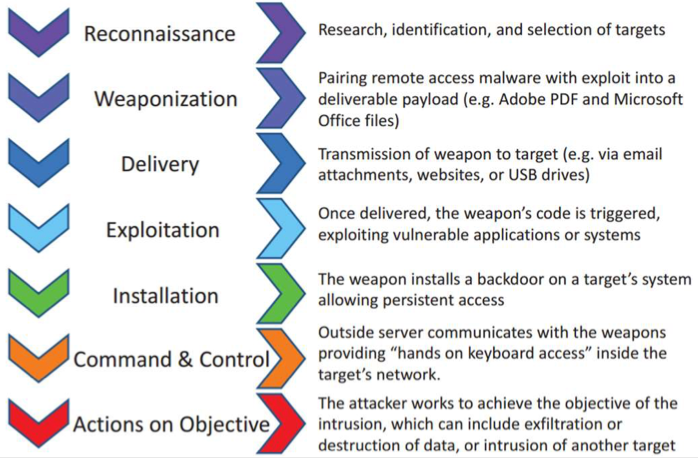
\includegraphics[width=\linewidth]{images/killchain.png}
  \caption{Cyber (intrusion) Kill Chain}
  \label{fig:killchain}
\end{figure}

From this brief introduction we can define he three pillars of security:
\begin{figure}[H]
  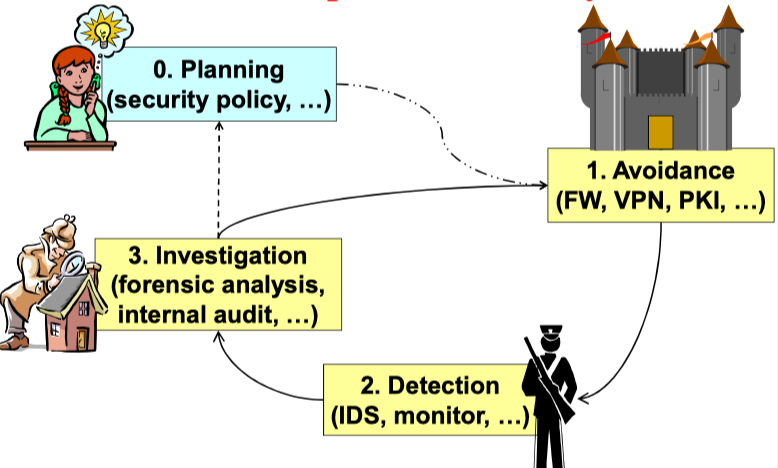
\includegraphics[width=\linewidth]{images/pillars.png}
  \caption{Pillars of Security}
  \label{fig:pillars}
\end{figure}
and we can define the main figures:
\begin{itemize}
  \item Hacker: Good and skilled
  \item Cracker: Bad but skilled
  \item Script Kiddie: Bad but NOT skilled
  \item Wannabe Lamer: Not good at all
\end{itemize}
%--------------------------------
%         END SLIDE 1           |
%--------------------------------















\end{document}
